%!Mode:: "TeX:UTF-8"
\documentclass[a4paper,11pt,UTF8]{ctexart}

\usepackage{indentfirst} %缩进
\usepackage{xeCJK}    %使用系统字体
\usepackage{fancyhdr} %自定义页眉页脚
\pagestyle{empty}                   %不设置页眉页脚
\usepackage{amsmath, amsthm, amssymb, amsfonts} %数学公式
\usepackage[a4paper,left=3cm,right=3cm,top=3cm,bottom=3cm]{geometry}
%\usepackage[tmargin=1in,bmargin=1in,lmargin=1.25in,rmargin=1.25in]{geometry}.
\usepackage{booktabs} %插入表格
\usepackage[section]{placeins} %避免浮动
\usepackage{listings} %插入代码
\usepackage{ctex}     %中文宏包
\usepackage[svgnames, table]{xcolor} %彩色表格
\usepackage{algorithm}          %伪代码
\usepackage{algorithmicx}
\usepackage{algpseudocode}
\usepackage{algorithm,algpseudocode,float}
\usepackage{lipsum}
\usepackage{enumitem}           %调整列举环境
\usepackage{url}
\usepackage{fontspec,xunicode}
\defaultfontfeatures{Mapping=tex-text} %如果没有它,会有一些 tex 特殊字符无法正常使用,比如连字符。

\usepackage{graphicx}
\graphicspath{{imgs/}}
\usepackage{physics}
%%%%%%%%%%%%%%%%%%%%%%%%%%%%%%%%%%%%%%%%%%%%%%%%%%%%%%%%%%%%%%%%
% 缩进及行间距
%%%%%%%%%%%%%%%%%%%%%%%%%%%%%%%%%%%%%%%%%%%%%%%%%%%%%%%%%%%%%%%%
\setlength{\parindent}{0pt} %重新定义缩进长度
\setlength{\baselineskip}{20pt}  %定义行间距
%\renewcommand{\baselinestretch}{1.1} %定义行间距

%%%%%%%%%%%%%%%%%%%%%%%%%%%%%%%%%%%%%%%%%%%%%%%%%%%%%%%%%%%%%%%%
% 列表设置
%%%%%%%%%%%%%%%%%%%%%%%%%%%%%%%%%%%%%%%%%%%%%%%%%%%%%%%%%%%%%%%%
\setenumerate{fullwidth,itemindent=\parindent,listparindent=\parindent,itemsep=0ex,partopsep=0pt,parsep=0ex}
\setenumerate[2]{label=\alph*),leftmargin=1.5em}  %二级item设置
\setitemize{itemindent=38pt,leftmargin=0pt,itemsep=-0.4ex,listparindent=26pt,partopsep=0pt,parsep=0.5ex,topsep=-0.25ex}
\setdescription{itemindent=38pt,leftmargin=0pt,itemsep=-0.4ex,listparindent=26pt,partopsep=0pt,parsep=0.5ex,topsep=-0.25ex}

%%%%%%%%%%%%%%%%%%%%%%%%%%%%%%%%%%%%%%%%%%%%%%%%%%%%%%%%%%%%%%%%
% 图的标题行间距设置
%%%%%%%%%%%%%%%%%%%%%%%%%%%%%%%%%%%%%%%%%%%%%%%%%%%%%%%%%%%%%%%%
\newcommand{\bottomcaption}{%
\setlength{\abovecaptionskip}{6pt}%
\setlength{\belowcaptionskip}{6pt}%
\caption}


%%%%%%%%%%%%%%%%%%%%%%%%%%%%%%%%%%%%%%%%%%%%%%%%%%%%%%%%%%%%%%%%
% 字体定义
%%%%%%%%%%%%%%%%%%%%%%%%%%%%%%%%%%%%%%%%%%%%%%%%%%%%%%%%%%%%%%%%
\setmainfont{Times New Roman}  %默认英文字体.serif是有衬线字体sans serif无衬线字体
\setmonofont{Consolas}
\setCJKmainfont[ItalicFont={楷体}, BoldFont={黑体}]{宋体}%衬线字体 缺省中文字体为
\setCJKsansfont{黑体}
\punctstyle{hangmobanjiao}
%-----------------------xeCJK下设置中文字体------------------------------%
\setCJKfamilyfont{song}{SimSun}                             %宋体 song
\newcommand{\song}{\CJKfamily{song}}
\setCJKfamilyfont{fs}{FangSong}                      %仿宋  fs
\newcommand{\fs}{\CJKfamily{fs}}
\setCJKfamilyfont{ktgb}{KaiTi}                      %楷体2312 ktgb
\newcommand{\ktgb}{\CJKfamily{ktgb}}
\setCJKfamilyfont{yh}{Microsoft YaHei}                    %微软雅黑 yh
\newcommand{\yh}{\CJKfamily{yh}}
\setCJKfamilyfont{hei}{SimHei}                              %黑体  hei
\newcommand{\hei}{\CJKfamily{hei}}
\setCJKfamilyfont{hwxk}{STXingkai}                                %华文行楷  hwxk
\newcommand{\hwxk}{\CJKfamily{hwxk}}
%------------------------------设置字体大小------------------------%
\newcommand{\shiyanbaogao}{\fontsize{36pt}{\baselineskip}\selectfont}
\newcommand{\chuhao}{\fontsize{42pt}{\baselineskip}\selectfont}     %初号
\newcommand{\xiaochuhao}{\fontsize{36pt}{\baselineskip}\selectfont} %小初号
\newcommand{\yihao}{\fontsize{28pt}{\baselineskip}\selectfont}      %一号
\newcommand{\erhao}{\fontsize{21pt}{\baselineskip}\selectfont}      %二号
\newcommand{\xiaoerhao}{\fontsize{18pt}{\baselineskip}\selectfont}  %小二号
\newcommand{\sanhao}{\fontsize{15.75pt}{\baselineskip}\selectfont}  %三号
\newcommand{\sihao}{\fontsize{14pt}{\baselineskip}\selectfont}       %四号
\newcommand{\xiaosihao}{\fontsize{12pt}{\baselineskip}\selectfont}  %小四号
\newcommand{\wuhao}{\fontsize{10.5pt}{\baselineskip}\selectfont}    %五号
\newcommand{\xiaowuhao}{\fontsize{9pt}{\baselineskip}\selectfont}   %小五号
\newcommand{\liuhao}{\fontsize{7.875pt}{\baselineskip}\selectfont}  %六号
\newcommand{\qihao}{\fontsize{5.25pt}{\baselineskip}\selectfont}    %七号

%%%%%%%%%%%%%%%%%%%%%%%%%%%%%%%%%%%%%%%%%%%%%%%%%%%%%%%%%%%%%%%%
% 图题字体大小相同
%%%%%%%%%%%%%%%%%%%%%%%%%%%%%%%%%%%%%%%%%%%%%%%%%%%%%%%%%%%%%%%%
\usepackage{caption}
\captionsetup{font={footnotesize}}   % footnotesize = 9pt
\captionsetup[lstlisting]{font={footnotesize}}

%%%%%%%%%%%%%%%%%%%%%%%%%%%%%%%%%%%%%%%%%%%%%%%%%%%%%%%%%%%%%%%%
% 重定义枚举编号为 1),2)...
%%%%%%%%%%%%%%%%%%%%%%%%%%%%%%%%%%%%%%%%%%%%%%%%%%%%%%%%%%%%%%%%
\renewcommand{\labelenumi}{\theenumi)}

%%%%%%%%%%%%%%%%%%%%%%%%%%%%%%%%%%%%%%%%%%%%%%%%%%%%%%%%%%%%%%%%
% 标题名称中文化
%%%%%%%%%%%%%%%%%%%%%%%%%%%%%%%%%%%%%%%%%%%%%%%%%%%%%%%%%%%%%%%%
\renewcommand\figurename{\hei 图}
\renewcommand\tablename{\hei 表}
\renewcommand\lstlistingname{\hei 代码}
\renewcommand{\algorithmicrequire}{\textbf{输入:}}
\renewcommand{\algorithmicensure}{\textbf{输出:}}
\newtheorem{define}{定义}

%%%%%%%%%%%%%%%%%%%%%%%%%%%%%%%%%%%%%%%%%%%%%%%%%%%%%%%%%%%%%%%%
% 代码设置
%%%%%%%%%%%%%%%%%%%%%%%%%%%%%%%%%%%%%%%%%%%%%%%%%%%%%%%%%%%%%%%%
\lstset{
 columns=fixed,
 numbers=left,                                        % 在左侧显示行号
 numberstyle=\tiny\color{gray},                       % 设定行号格式
 frame=single,                                        % 单线背景边框
 breaklines=true,                                     % 设定LaTeX对过长的代码行进行自动换行
 keywordstyle=\color[RGB]{40,40,255},                 % 设定关键字颜色
 numberstyle=\footnotesize\color{darkgray},
 commentstyle=\it\color[RGB]{0,96,96},                % 设置代码注释的格式
 stringstyle=\rmfamily\slshape\color[RGB]{128,0,0},   % 设置字符串格式
 showstringspaces=false,                              % 不显示字符串中的空格
 language=java,                                        % 设置语言
 basicstyle=\linespread{1.0}\xiaowuhao\ttfamily,                      % 字体字号
 %lineskip=10pt,
 %baselinestretch=1,
}

%%%%%%%%%%%%%%%%%%%%%%%%%%%%%%%%%%%%%%%%%%%%%%%%%%%%%%%%%%%%%%%%
% 伪代码分页
%%%%%%%%%%%%%%%%%%%%%%%%%%%%%%%%%%%%%%%%%%%%%%%%%%%%%%%%%%%%%%%%
\makeatletter
\renewcommand{\ALG@name}{算法}
\newenvironment{breakablealgorithm}
  {% \begin{breakablealgorithm}
   \begin{center}
     \refstepcounter{algorithm}% New algorithm
     \hrule height.8pt depth0pt \kern2pt% \@fs@pre for \@fs@ruled
     \renewcommand{\caption}[2][\relax]{% Make a new \caption
       {\raggedright\textbf{\ALG@name~\thealgorithm} ##2\par}%
       \ifx\relax##1\relax % #1 is \relax
         \addcontentsline{loa}{algorithm}{\protect\numberline{\thealgorithm}##2}%
       \else % #1 is not \relax
         \addcontentsline{loa}{algorithm}{\protect\numberline{\thealgorithm}##1}%
       \fi
       \kern2pt\hrule\kern2pt
     }
  }{% \end{breakablealgorithm}
     \kern2pt\hrule\relax% \@fs@post for \@fs@ruled
   \end{center}
  }
\makeatother

% =============================================
% Part 1 Edit the info
% =============================================


\title{计数器及其应用}
\author{戴佳乐 \quad PB18020556 \quad 苗立扬 \quad PB19000132}

\newcommand{\course}{电子线路实验(1)}
\newcommand{\newtitle}{计数器及其应用}

% =============================================
% Part 1 Main document
% =============================================
\begin{document}
\maketitle

% =============================================
% Part 2 Main document
% =============================================

%
\newcommand{\p}{\par}
\newcommand{\np}{\par\noindent}
%
\newcommand{\expa}{分别验证74LS90实现2、5、10进制计数器}
\newcommand{\expb}{用一块74LS90实现8进制的计数器}
\newcommand{\expc}{用两块74LS90实现100进制的计数器}
\newcommand{\expd}{用两块74LS90实现60进制的计数器(数字钟计数)}
\newcommand{\chip}{数据选择器74LS151}

\newcommand{\CI}{C\negthinspace I}
\newcommand{\CO}{C\negthinspace O}
%

\section{实验目的}

(1)掌握中规模集成电路的功能及使用方法。\\
(2)学习用“反馈归零法” 构成N进制计数器的方法。\\
(3)学会中规模集成电路的分析方法、设计方法和测试方法。\\



\section{实验原理}
(1)计数器按触发信号的来源不同,可分为同步计数器和异步计数器。\\
(2)同步计数器是指计数器内所有的触发器共同使用同一个输入的时钟脉冲信号,在同一个时刻翻转,计数速度快。\\
(3)异步计数器是指计数器内各触发器的输入时钟信号的来源不同,各电路的翻转时刻也不一样,因此计数速度较慢。但由于使用了多组计数器的组合,该计数电路能够扩展计数电路的计数范围。\\

本次实验,我们使用74LS90芯片用作计数器。该芯片内集成了一个二进制计数器与与一个五进制计数器,可以组合成为任何小于10的计数器。该芯片包含四个输出引脚,两个时钟脉冲引脚与两个清零端与置9端,可以满足我们在该实验中对芯片的要求。

\begin{figure}[H]
  \centering
  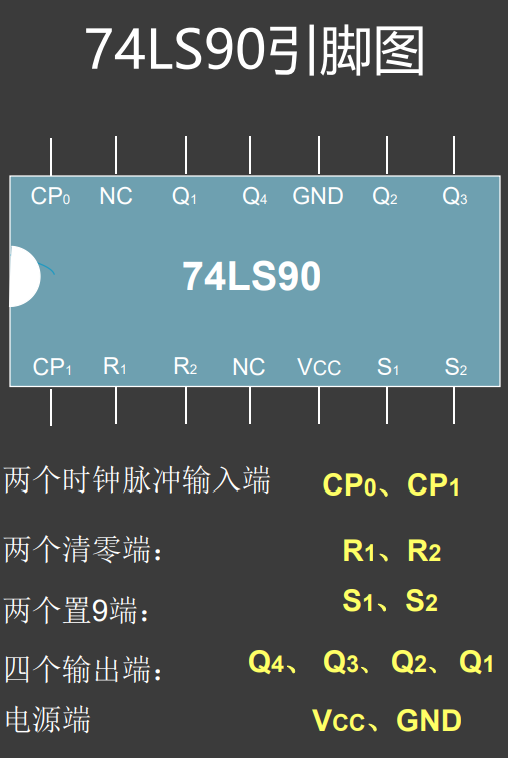
\includegraphics[width=6cm]{jsq1}
  \caption{74LS90引脚图}
  \label{fig:jsq1}
\end{figure}

\begin{figure}[H]
  \centering
  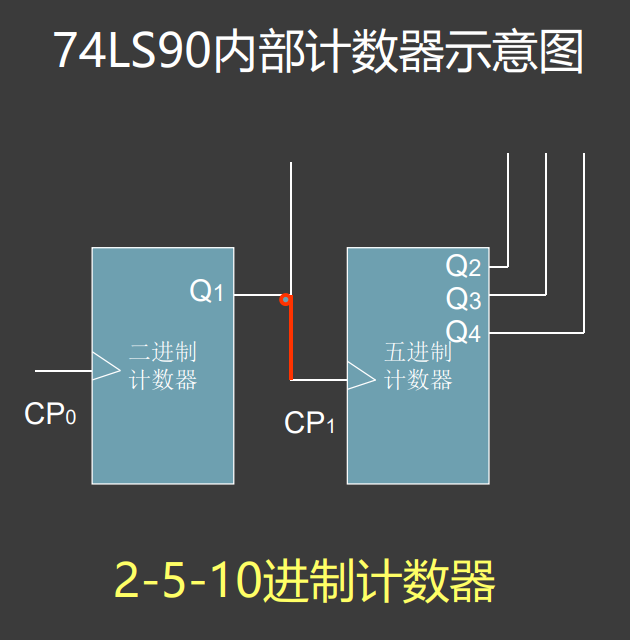
\includegraphics[width=6cm]{jsq2}
  \caption{74LS90内部计数器示意图}
  \label{fig:jsq2}
\end{figure}





\section{实验内容、步骤与结果}
 \subsection{实验一:\expa}
\subsubsection{二进制计数}
	按PPT所示图1端口说明,将外部时钟脉冲接入14端口,NC端口置空,两个清零端与置9端各接地至少一个,1端口接地,则12($Q_0$)端口输出为2进制计数

\subsubsection{五进制计数}
	按PPT所示图1端口说明,将外部时钟脉冲接入1端口,NC端口置空,两个清零端与置9端各接地至少一个,14端口接地,则8、9、11($Q_1, Q_2, Q_3$)端口输出5进制计数
	
\subsubsection{十进制计数}
	按PPT所示图1端口说明,将外部时钟脉冲接入14端口,NC端口置空,两个清零端与置9端各接地至少一个,并将2进制端口12与五进制时钟脉冲端口1相连,组合为异步计数器,则12、8、9、11($Q_0,Q_1, Q_2, Q_3$)端口输出10进制计数
	
	
	
	
	
	电路状态图如实验报告所示


 \subsection{实验二:\expb}
 由八进制计数的特点,我们只需作自然截断,使电路在1000状态置零即可。所以我们可以将$Q_3$端口与两置零端相连,使电路在计数8的时候归零,由此实现八进制。
 
 电路图如图3所示,电路状态图如实验报告所示。
 \begin{figure}[H]
  \centering
  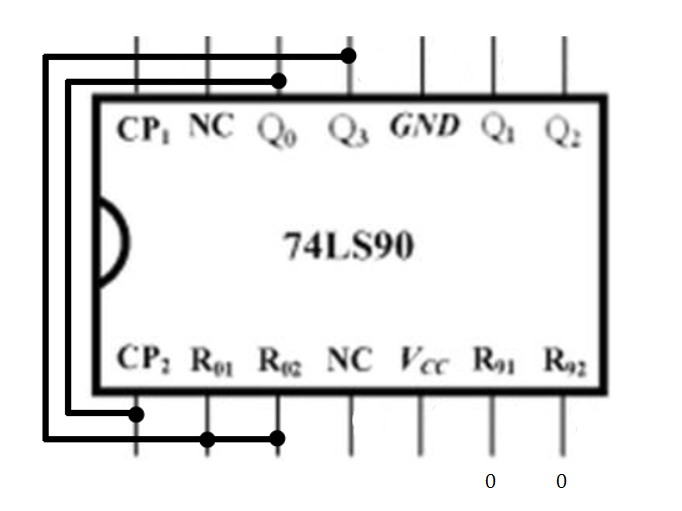
\includegraphics[width=8cm]{jsq3}
  \caption{74LS90实现8进制计数器}
  \label{fig:jsq3}
 \end{figure}
 
 \subsection{实验三:\expc}
 多个计数器计数范围扩展时,我们只需将前一计数器的最高位输出接入后一计数器作为后裔计数器的时钟脉冲即可,如同2进制+5进制=10进制的电路改造。
 
 电路图如图4所示,状态图如实验报告所示。
 \begin{figure}[H]
  \centering
  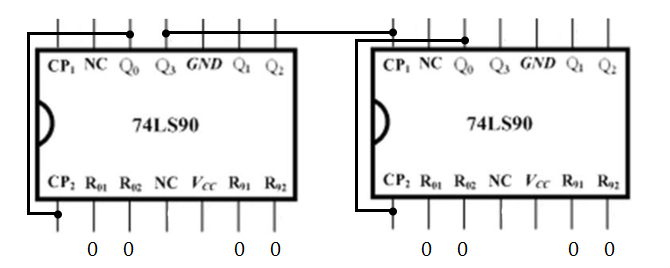
\includegraphics[width=14cm]{jsq4}
  \caption{两块74LS90实现100进制计数器}
  \label{fig:jsq4}
 \end{figure}

 \subsection{实验四:\expd}
 在实验三的基础上,我们考虑将后一位计数芯片改为六进制即可。实验芯片线路如图5所示。
 \begin{figure}[H]
  \centering
  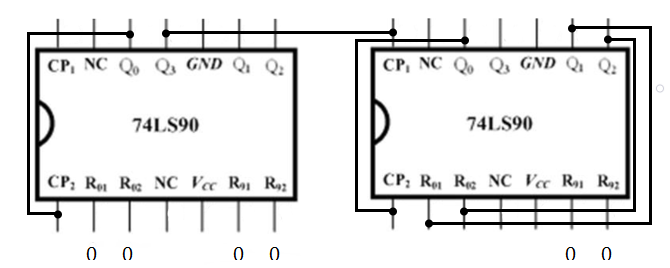
\includegraphics[width=14cm]{jsq5}
  \caption{数字钟计数}
  \label{fig:jsq5}
 \end{figure}








  


  
 

\section{总结}
通过这次实验,本组同学掌握了中规模集成电路的功能及使用方法,
学习了用“反馈归零法”构成N进制计数器的方法,
学会了中规模集成电路的分析方法、设计方法和测试方法。


 










\end{document}
